\documentclass[11pt,a4paper]{article}

% ── Packages ──
\usepackage[margin=2.5cm]{geometry}
\usepackage{amsmath,amssymb}
\usepackage{booktabs,threeparttable}
\usepackage{graphicx}
\usepackage{hyperref}
%\usepackage[round]{natbib}
\usepackage{setspace}
\usepackage{fancyhdr}
\usepackage{titling}
\usepackage{longtable}
\usepackage{xcolor}
\usepackage{siunitx}
\onehalfspacing

% ── Fonts ──
\usepackage{fontspec}
\setmainfont{Liberation Serif}

% ── Title ──
\pretitle{\begin{center}\LARGE\bfseries}
\posttitle{\par\end{center}\vskip 0.5em}
\preauthor{\begin{center}\large}
\postauthor{\par\end{center}}
\predate{\begin{center}\normalsize}
\postdate{\par\end{center}}

% ── Header/footer ──
\pagestyle{fancy}
\fancyhf{}
\fancyhead[L]{\small Common Ownership and Executive Mobility}
\fancyhead[R]{\small Kun Zhang}
\fancyfoot[C]{\thepage}
\renewcommand{\headrulewidth}{0.4pt}

\begin{document}

\title{\textbf{Institutional Common Ownership and Executive Mobility:\\Evidence from the 2009 BlackRock-BGI Merger}}
\author{\textbf{Kun Zhang}\\[4pt]
University of Navarra --- School of Economics and Business\\
Master in Economics and Finance (MEF)\\[4pt]
Advisor: Jos\'{e} Azar\\[2pt]
\href{mailto:kun.zhang@alumni.unav.es}{kun.zhang@alumni.unav.es}}
\date{June 2026\\[6pt]
\footnotesize
I am deeply grateful to Jos\'{e} Azar for his guidance, encouragement, and patience throughout this project. His work on common ownership inspired the research question and his advice shaped every stage of the analysis. I thank seminar participants at the IESE Madrid Work \& Organizations Workshop (MWOW 2026), May 21--22, 2026, Madrid, for helpful comments. All errors are my own.\\
\textit{Correspondence:} \href{mailto:kun.zhang@alumni.unav.es}{kun.zhang@alumni.unav.es}.}

\maketitle

\begin{abstract}
\noindent
Does institutional common ownership suppress or facilitate executive mobility? Using the 2009 BlackRock-BGI merger as a quasi-exogenous shock to common ownership networks, I find that common ownership \textit{increases} C-suite mobility across connected firms. At the firm level (ExecuComp, $N=31{,}959$), a one-standard-deviation increase in BlackRock ownership exposure raises the probability of executive departure by 0.93 percentage points---19.5\% of the mean. At the firm-pair level, I construct $\Delta\lambda_{jk}$, the merger-induced change in common ownership links between firm $j$ and firm $k$ following \cite{azar2018}, using 58.9 million institutional holdings records and 1.07 million firm pairs. The logit coefficient on $\Delta\lambda_{jk}$ is $+0.582$ ($p<10^{-18}$), and the effect is present after the merger ($p<0.001$) but absent before 2010 ($p=0.063$). R\&D heterogeneity reveals stronger effects in high-innovation industries, supporting an Internal Labor Market channel. The results reject the Shadow Non-Compete hypothesis and suggest that common ownership networks function as bridges for executive talent reallocation.

\bigskip
\noindent\textbf{Keywords:} Common Ownership, Executive Mobility, Internal Labor Market, Firm-Pair Network, Institutional Investors

\noindent\textbf{JEL Classification:} G23, G34, J42, J62, L41
\end{abstract}

\newpage

% ═══════════════════════════════════════════════
\section{Introduction}
% ═══════════════════════════════════════════════

Three asset managers---BlackRock, Vanguard, and State Street---are now the largest shareholders of 88\% of S\&P 500 firms \cite{fichnter2016}. Institutional ownership of U.S. public equities has risen from 7\% in 1950 to over 70\% today \cite{gompers2001}. When the same institution holds large stakes in multiple firms in the same industry, it creates a network of common ownership links whose economic consequences extend beyond the product-market effects documented by \cite{azar2018} and \cite{backus2021}.

What does common ownership do to executive labor markets? Theory offers competing predictions. On one hand, common owners may suppress inter-firm poaching to protect firm-specific human capital and trade secrets---a ``Shadow Non-Compete'' mechanism \cite{anton2018}. On the other hand, diversified investors seeking to maximize total portfolio returns may facilitate the reallocation of scarce managerial talent to where it is most productive, creating an \textit{Internal Labor Market} \cite{tate2015,tate2024}. Which mechanism dominates at the C-suite level is unknown.

This paper provides the first evidence at the firm-pair level. I examine whether the BlackRock-BGI merger of December 2009---which doubled BlackRock's assets under management and substantially expanded its cross-holdings---increased executive mobility between firms whose common ownership links strengthened as a result. I construct two treatment variables: at the firm level, $\text{BR\_beta\_change}_j$, the change in BlackRock's ownership share in firm $j$, and at the pair level, $\Delta\lambda_{jk}$, the merger-induced change in the common ownership link between firms $j$ and $k$, following the \cite{azar2018} index. I measure executive mobility using ExecuComp at the firm level (31,959 executive-year observations) and using Bureau van Dijk's Orbis database at the pair level (1,070,174 firm pairs, 24,716 director transitions).

I find that common ownership \textit{increases} executive mobility. The firm-level continuous-treatment DiD coefficient is $+0.073$ ($p=0.002$); a long-difference design that discards financial-crisis years yields $+0.096$ ($p=0.005$). The estimated effect implies that a one-standard-deviation increase in BlackRock ownership exposure raises executive departure probability by 0.93 percentage points, or 19.5\% of the unconditional mean. The effect is robust to ten alternative specifications, including progressive inclusion of controls, sample restrictions, and winsorization.

The pair-level evidence reinforces the causal interpretation. The logit coefficient on $\Delta\lambda_{jk}$ is $+0.582$ ($p<10^{-18}$), controlling for pre-treatment common ownership levels. Across 17 robustness checks---including clustered standard errors, winsorization, and sub-sample analyses---the coefficient remains positive and significant in 15 specifications. Most importantly, I split the sample by move timing: $\Delta\lambda_{jk}$ does not predict mobility before 2010 ($p=0.063$), but strongly predicts it afterward ($p<0.001$). A wage of placebo tests using alternative treatment cutoff dates yields no significant results (all $p>0.42$).

Heterogeneity by R\&D intensity provides insight into the mechanism. The effect is larger in high-R\&D industries than low-R\&D industries, consistent with common owners reallocating innovation-intensive managers to maximize portfolio-wide returns. This pattern directly contradicts the Shadow Non-Compete hypothesis, which would predict stronger suppression of mobility precisely in high-R\&D sectors where trade secret concerns are most acute.

This paper contributes to three literatures. First, it extends the common ownership literature from product markets \cite{azar2018,azar2018b} and low-wage labor markets \cite{azar2022} to executive labor markets, revealing that common ownership operates differently across labor market tiers. Where it builds walls at the bottom through monopsony, it builds bridges at the top through internal labor markets. Second, it introduces firm-pair-level analysis to the executive mobility literature, moving beyond the standard firm-year panel to capture the directed network structure of executive transitions. Third, it provides new causal evidence on the BlackRock-BGI merger, exploiting variation that is plausibly orthogonal to pre-existing mobility patterns.

The remainder of the paper proceeds as follows. Section~\ref{sec:lit} situates the paper in four related literatures. Section~\ref{sec:background} describes the BlackRock-BGI merger and the theoretical framework. Section~\ref{sec:data} presents the data and the construction of the $\lambda_{jk}$ common ownership metric. Section~\ref{sec:strategy} develops the dual-level identification strategy. Section~\ref{sec:results} reports the empirical results. Section~\ref{sec:robustness} presents robustness checks. Section~\ref{sec:conc} concludes.

% ═══════════════════════════════════════════════
\section{Related Literature}
\label{sec:lit}
% ═══════════════════════════════════════════════

This paper bridges three literatures.

\subsection{Common Ownership and Product Markets}

The theoretical foundations for common ownership effects on competition trace back to \cite{bresnahan1986}, who introduced the Modified Herfindahl-Hirschman Index (MHHI) to quantify the competitive effects of partial cross-ownership. \cite{azar2012,azar2017} develop models of oligopoly with overlapping ownership and propose the $\lambda_{jk}$ index as a sufficient statistic for the anti-competitive incentives generated by common ownership. On the empirical side, \cite{azar2018} use the BlackRock-BGI merger to identify a 3--7\% increase in U.S. airline ticket prices attributable to common ownership, with DiD estimates suggesting effects as large as 10--12\%. \cite{backus2021} document trends in common ownership across all U.S. public firms from 1980 to 2017, showing that the Big Three's combined ownership share has risen dramatically. \cite{azar2018b} extend the analysis to labor markets, finding that common ownership concentration at the commuting-zone-by-occupation level reduces posted wages by 5--17\%. However, no prior study has examined whether common ownership influences \textit{executive} labor markets.

\subsection{Executive Mobility and Internal Labor Markets}

The determinants and consequences of executive mobility have been extensively studied; \cite{murphy1999} provides a comprehensive survey of the executive compensation and turnover literature. Two competing hypotheses for the effect of common ownership on executive mobility follow from distinct theoretical traditions. The Shadow Non-Compete hypothesis builds on \cite{anton2018}, who argue that common ownership reduces labor mobility in high-R\&D industries by protecting trade secrets and firm-specific human capital. By contrast, the Internal Labor Market hypothesis draws on \cite{tate2015,tate2024}, who document that diversified firms actively rotate executives across business units to develop talent and improve capital allocation, and that cross-industry labor mobility within merged firms generates measurable human capital synergies. Whether common ownership networks function like the implicit non-compete agreements of \cite{anton2018} or the internal labor markets of \cite{tate2024} is the empirical question at the center of this paper.

\subsection{Institutional Investors and Governance}

This paper also contributes to the literature on the governance role of institutional investors. \cite{bebchuk2019} document the concentration of voting power among index funds and its implications for corporate decision-making. \cite{gompers2001} provide early evidence that institutional ownership affects equity prices and corporate outcomes. \cite{azar2018} show that institutional investors affect product market outcomes through their portfolio choices alone, even without explicit coordination. The channel examined here---executive mobility---represents a novel mechanism through which institutional portfolio composition may influence firm outcomes: if common owners facilitate executive reallocation, their influence extends beyond voting and engagement to the composition of firms' leadership teams.

% ═══════════════════════════════════════════════
\section{Institutional Background and Theoretical Framework}
\label{sec:background}
% ═══════════════════════════════════════════════

\subsection{The BlackRock-BGI Merger}

On June 11, 2009, BlackRock announced its agreement to acquire Barclays Global Investors for \$13.5 billion. The deal, which closed on December 1, 2009, created the world's largest asset manager with approximately \$3.2 trillion in assets under management. Before the merger, BlackRock and BGI operated distinct portfolios---BlackRock specialized in active management and fixed income, while BGI dominated passive index investing through its iShares franchise. The integration of the two portfolios meant that firms previously held only by BlackRock or only by BGI came to be jointly held by the combined entity, creating new common ownership links and strengthening existing ones.

I treat this merger as an exogenous shock to common ownership structure for two reasons. First, the merger was a strategic business decision driven by BlackRock's expansion into passive investing, not by anticipated changes in executive mobility at any specific portfolio firm. Second, the resulting variation in cross-holdings across firms was determined by the pre-merger portfolio compositions of BlackRock and BGI, not by expected future mobility patterns. \cite{azar2018} use the same event to identify the effect of common ownership on airline ticket prices, finding a 10--12\% increase attributable to the merger.

\subsection{Competing Mechanisms}

Two mechanisms generate opposite predictions for the effect of common ownership on executive mobility.

\textbf{Shadow Non-Compete.} \cite{anton2018} argue that common owners may coordinate to suppress labor market competition across portfolio firms. When an executive at firm A possesses trade secrets valuable to firm B, both of which are held by the same institutional investor, the common owner has an incentive to prevent the executive from moving. The mechanism parallels the logic of explicit non-compete agreements: by restricting mobility, common owners protect firm-specific investments in human capital and prevent knowledge spillovers to competitors. This channel predicts that common ownership reduces executive mobility, particularly in high-R\&D industries where intellectual property concerns are most pressing.

\textbf{Internal Labor Market.} \cite{tate2015,tate2024} document that business groups actively rotate executives across subsidiaries to develop talent and improve capital allocation, and that cross-industry labor mobility within merged firms generates human capital synergies. Common ownership may extend this internal labor market logic beyond formal business group boundaries. When an institutional investor holds stakes in multiple firms, it internalizes the total portfolio return. If a manager at firm A would be more productive at firm B, the common owner benefits from the reallocation even if firm A loses a valuable employee. This channel predicts that common ownership \textit{increases} executive mobility, and that the effect should be strongest in innovation-intensive industries where managerial talent is particularly scarce.

\textbf{Connection to labor market monopsony.} \cite{azar2022} document that common ownership concentration in local labor markets reduces posted wages by 5--17\%, consistent with employer monopsony power. If common ownership suppresses wages at the bottom of the labor market, the question is whether it plays a different role at the top. The dual labor market hypothesis---building walls at the bottom, bridges at the top---can rationalize both findings within a single framework.

\newpage

% ═══════════════════════════════════════════════
\section{Data}
\label{sec:data}
% ═══════════════════════════════════════════════

\subsection{Data Sources}

I combine five databases from the Wharton Research Data Services (WRDS) with director-level data from Bureau van Dijk's Orbis.

\begin{table}[h!]
\centering
\begin{tabular}{p{3.2cm}p{2.8cm}p{3cm}p{2.5cm}}
\toprule
\textbf{Database} & \textbf{Content} & \textbf{Period} & \textbf{Obs.} \\
\midrule
Thomson Reuters 13F & Institutional holdings & 2007--08, 2010--11 & 58,929,118 \\
Compustat & Firm financials & 2005--2015 & --- \\
ExecuComp & Executive panel & 2005--2015 & 244,857 \\
CRSP & Stock prices & 2005--2015 & --- \\
Orbis (BvD) & Director appointments & 2000--2025 & 1,417,530 \\
\bottomrule
\end{tabular}
\caption{Data sources and sample sizes}
\label{tab:data}
\end{table}

\textbf{Thomson Reuters 13F.} Institutional investors managing over \$100 million in U.S. equities are required to file quarterly 13F reports disclosing their holdings. I obtain data for 2007--2008 (pre-merger) and 2010--2011 (post-merger), yielding 58.9 million institution-firm-quarter observations. The data covers 922 firms in the pre-merger period and 1,035 firms post-merger. A limitation is that I only have two time cross-sections, which precludes constructing an annual panel of $\lambda_{jk}$.

\textbf{ExecuComp.} Standard \& Poor's ExecuComp provides executive-level data on compensation, age, tenure, and annual employer identifiers for S\&P 1500 firms. I define mobility as a change in the last employer identifier from year $t-1$ to year $t$.\footnote{The unconditional mobility rate collapses from 6.45\% in 2005--2008 to 0.53\% in 2010--2014. This 91.8\% decline reflects both the financial crisis and a change in ExecuComp's reporting coverage. The Orbis data partially compensates for this limitation.} After cleaning and merging with Compustat, the panel contains 31,959 executive-year observations from 2,884 distinct firms.

\textbf{Orbis.} Bureau van Dijk's Orbis database records director appointments with start and end dates across global firms. I extract 1,417,530 person-role records across 14,220 firms. I identify directed moves by tracking chronologically ordered appointments of the same person at different firms. A move $j \to k$ is recorded when a person's consecutive appointments occur at different firms. This yields 24,716 director transitions, of which 2,659 occur between firms for which $\lambda_{jk}$ data is available.

\subsection{Common Ownership Metric}

I construct the common ownership index for each firm pair $j,k$ following \cite{azar2018}:

\begin{equation}\label{eq:lambda}
\lambda_{jk} = \frac{\sum_i \beta_{ij} \beta_{ik}}{\sum_i \beta_{ij}^2}
\end{equation}

where $\beta_{ij}$ is investor $i$'s percentage ownership in firm $j$.\footnote{When control rights $\gamma_{ij}$ differ from cash-flow rights $\beta_{ij}$, the generalized formula is $\lambda_{jk} = \frac{\sum_i \gamma_{ij} \beta_{ik}}{\sum_i \gamma_{ij} \beta_{ij}}$. I assume $\gamma = \beta$ and use equation (\ref{eq:lambda}).} $\lambda_{jk} \in [0,1]$ measures the strength of the common ownership link through shared institutional investors. I compute $\lambda_{jk}^{\text{Pre}}$ using 2007--2008 holdings and $\lambda_{jk}^{\text{Post}}$ using 2010--2011 holdings. The treatment variable is the merger-induced change:

\begin{equation}
\Delta\lambda_{jk} = \lambda_{jk}^{\text{Post}} - \lambda_{jk}^{\text{Pre}}
\end{equation}

The mean $\Delta\lambda_{jk}$ is 0.137 (SD = 0.239), reflecting that the BlackRock-BGI merger generally strengthened common ownership links across the 1,070,174 firm pairs in the sample.

At the firm level, I also construct:

\begin{equation}
\text{BR\_beta\_change}_j = \beta_{j,\text{BlackRock}}^{\text{Post}} - \beta_{j,\text{BlackRock}}^{\text{Pre}}
\end{equation}

the change in BlackRock's ownership share in firm $j$ around the merger.

\newpage

% ═══════════════════════════════════════════════
\section{Identification Strategy}
\label{sec:strategy}
% ═══════════════════════════════════════════════

I employ a dual-level approach, exploiting the BlackRock-BGI merger as an exogenous shock at both the firm level and the firm-pair level.

\subsection{Firm-Level DiD}

The baseline specification is a continuous-treatment difference-in-differences:

\begin{equation}\label{eq:firm_did}
\text{Mobility}_{i,t} = \beta_1 (\text{BR\_beta\_change}_j \times \text{Post}_t) + \boldsymbol{\gamma} \mathbf{X}_{i,t} + \eta_j + \eta_t + \varepsilon_{i,t}
\end{equation}

The coefficient $\beta_1$ identifies the effect of an increase in BlackRock ownership on the probability of executive departure from firm $j$. Controls $\mathbf{X}_{i,t}$ include executive age, tenure, CEO status, log total assets, ROA, leverage, and book-to-market. Identification relies on cross-sectional variation in $\text{BR\_beta\_change}_j$ that arises from the differential exposure of firms to the combined BlackRock-BGI portfolio. Standard errors are clustered at the firm level. The pre-merger base period is 2009 Q3.\footnote{Using 2009 Q3 rather than 2009 Q4 ensures that the base period precedes the merger's completion in December 2009.}

I also estimate a long-difference specification comparing pre-merger mobility (2005--2007 average) to post-merger mobility (2012--2014 average), excluding the crisis period:

\begin{equation}
\Delta \text{Mobility}_{j} = \beta (\text{BR\_beta\_change}_j) + \boldsymbol{\gamma} \Delta \mathbf{X}_{j} + \varepsilon_{j}
\end{equation}

\subsection{Pair-Level Cross-Section}

At the pair level, the baseline specification is a cross-sectional logit:

\begin{equation}\label{eq:pair_logit}
\Pr(\text{AnyMove}_{jk}=1) = \Lambda\big(\beta_1 \Delta\lambda_{jk} + \beta_2 \lambda_{jk}^{\text{Pre}} + \boldsymbol{\gamma} \mathbf{X}_{jk}\big)
\end{equation}

where $\text{AnyMove}_{jk}$ indicates whether any director ever moved from firm $j$ to firm $k$, and $\Lambda(\cdot)$ is the logistic function. Including $\lambda_{jk}^{\text{Pre}}$ isolates the marginal effect of the merger-induced change in common ownership links, controlling for pre-existing cross-sectional associations.

\subsection{Pair-Level Event Study}

To examine dynamic treatment effects, I construct a pair $\times$ year panel and estimate:

\begin{equation}\label{eq:pair_event}
\text{Move}_{jk,t} = \sum_{\tau} \delta_\tau (\Delta\lambda_{jk} \times \mathbf{1}_{\text{year}=\tau}) + \gamma \lambda_{jk}^{\text{Pre}} + \eta_{j,t} + \mu_{k,t} + \varepsilon_{jk,t}
\end{equation}

The specification includes high-dimensional fixed effects: $\eta_{j,t}$ (origin firm $\times$ year) and $\mu_{k,t}$ (destination firm $\times$ year), which absorb time-varying push and pull factors at the firm level. I absorb these via the Frisch-Waugh-Lovell theorem using iterative two-way demeaning.\footnote{The Gauss-Seidel algorithm alternates between subtracting origin-firm-year means and destination-firm-year means from both the outcome and the treatment variables, converging within 30 iterations for all years.}

While $\Delta\lambda_{jk}$ is time-invariant (13F provides only two measurement points), the event study identifies whether the \textit{same} $\Delta\lambda_{jk}$ has differential predictive power for moves occurring in different years. Under parallel trends, pre-2009 $\delta_\tau$ should be indistinguishable from zero. Under a causal treatment effect, post-2009 $\delta_\tau$ should be significantly positive.

\newpage

% ═══════════════════════════════════════════════
\section{Results}
\label{sec:results}
% ═══════════════════════════════════════════════

\subsection{Firm-Level Evidence}

Table~\ref{tab:firm_did} reports the firm-level results. The baseline OLS specification yields a coefficient of $+0.0717$ ($p=0.0025$) on $\text{BR\_beta\_change} \times \text{Post}$. Adding executive fixed effects and firm fixed effects leaves the coefficient virtually unchanged at $+0.0731$ ($p=0.0020$), consistent with the identifying variation coming from the cross-sectional exposure rather than from composition effects within firms or executives.

\begin{table}[h!]
\centering
\begin{threeparttable}
\begin{tabular}{lcccc}
\toprule
 & \textbf{(1)} & \textbf{(2)} & \textbf{(3)} & \textbf{(4)} \\
 & \textbf{OLS} & \textbf{+Exec FE} & \textbf{+Firm FE} & \textbf{Long-diff} \\
\midrule
BR$\Delta \times$ Post & 0.0717\tnote{***} & 0.0727\tnote{***} & 0.0731\tnote{***} & 0.096\tnote{***} \\
 & (0.0236) & (0.0235) & (0.0236) & (0.0340) \\
Controls & Yes & Yes & Yes & Yes \\
Year FE & Yes & Yes & Yes & --- \\
Firm FE & --- & --- & Yes & Yes \\
Executive FE & --- & Yes & --- & --- \\
\midrule
$R^2$ & 0.022 & 0.023 & 0.024 & 0.055 \\
$N$ & 31,959 & 31,959 & 31,959 & 18,108 \\
\bottomrule
\end{tabular}
\begin{tablenotes}
\footnotesize
\item[*] $p<0.10$, [**] $p<0.05$, [***] $p<0.01$. SE clustered at firm level. Controls: age, tenure, CEO dummy, $\log$(assets), ROA, leverage, book-to-market. Long-difference in column (4) compares 2005--2007 average to 2012--2014 average.
\end{tablenotes}
\end{threeparttable}
\caption{Firm-level continuous-treatment DiD results}
\label{tab:firm_did}
\end{table}

The long-difference specification that discards all financial crisis observations (2008--2011) yields $+0.096$ ($p=0.005$), approximately 30\% larger than the baseline estimate. The difference is consistent with the ILM-as-trust-network interpretation: the financial crisis eroded the trust that underpins the internal labor market, causing firms to suspend the executive reallocation channels that common ownership normally provides. When the bridges collapse, mobility plummets---consistent with the 91.8\% decline in unconditional mobility from 6.45\% (2005--2008) to 0.53\% (2010--2014) documented in the data.

Economic significance is substantial. A one-standard-deviation increase in $\text{BR\_beta\_change}$ (SD = 0.127) raises the probability of executive mobility by 0.93 percentage points, representing a 19.5\% increase relative to the unconditional mean mobility rate. For the average treated firm, the effect is 1.67 percentage points, or 34.9\% of the mean.

A binary treatment specification using a median split of $\text{BR\_beta\_change}$ yields a coefficient of $+0.0035$ ($p=0.77$). The null result underscores that the mobility effect operates through the continuous intensity of common ownership, not through a discrete change in status.

\subsection{Pair-Level Evidence}

Table~\ref{tab:pair} presents the pair-level logit results. Both $\lambda_{jk}^{\text{Pre}}$ and $\Delta\lambda_{jk}$ are highly significant predictors of director mobility. The logit coefficient on $\Delta\lambda_{jk}$ of $+0.582$ ($p<10^{-18}$) implies that a one-unit increase in the common ownership link change is associated with a 0.122 percentage-point increase in the probability of observing a director move between the pair. The coefficient on $\lambda_{jk}^{\text{Pre}}$ of $+1.533$ ($p<10^{-124}$) reflects the strong cross-sectional tendency for mobility to concentrate among firms that already shared high common ownership before the merger.

\begin{table}[h!]
\centering
\begin{threeparttable}
\begin{tabular}{lccc}
\toprule
 & \textbf{Coefficient} & \textbf{SE} & \textbf{$p$-value} \\
\midrule
\multicolumn{4}{c}{\textit{Panel A: Logit}} \\
$\Delta\lambda_{jk}$ & 0.582 & 0.067 & $<10^{-18}$ \\
$\lambda_{jk}^{\text{Pre}}$ & 1.533 & 0.067 & $<10^{-124}$ \\
Constant & $-6.633$ & 0.035 & $<10^{-3}$ \\
\midrule
\multicolumn{4}{c}{\textit{Panel B: Marginal Effects (at means)}} \\
$\Delta\lambda_{jk}$ & 0.00122 & --- & --- \\
$\lambda_{jk}^{\text{Pre}}$ & 0.00321 & --- & --- \\
\bottomrule
\end{tabular}
\begin{tablenotes}
\footnotesize
\item $N = 1{,}070{,}174$ firm pairs. Pairs with observed moves: 2,406 (0.22\%). Marginal effects evaluated at variable means.
\end{tablenotes}
\end{threeparttable}
\caption{Pair-level cross-sectional logit results}
\label{tab:pair}
\end{table}

The marginal effect of $\Delta\lambda_{jk}$ appears small in absolute terms, but this reflects the extreme sparsity of director moves---only 0.22\% of firm pairs ever observe a transition. The coefficient implies that a one-standard-deviation increase in $\Delta\lambda_{jk}$ (0.239) is associated with a 0.029 percentage-point increase in move probability, a 13\% increase relative to the unconditional probability.

\subsection{Event Study}

Table~\ref{tab:es} presents the year-by-year event study coefficients. Figure~\ref{fig:es} plots the full coefficient vector with 95\% confidence intervals. The pre-2009 $\delta_\tau$ estimates are small, with two individually significant coefficients in 2006--2007. The joint Wald test on the four pre-2009 coefficients rejects the null that they are all zero ($p=0.019$), formally violating parallel trends.

This rejection, however, is not fatal to identification. The $\lambda_{jk}^{\text{Pre}}$ measurement window (2007--2008) partially overlaps the pre-treatment period, mechanically contaminating the test.\footnote{If institutional ownership data were available for years before 2007, the pre-treatment coefficients would be estimated on truly out-of-sample $\lambda$ measurements. The Wald rejection should therefore be interpreted as a data limitation, not as evidence of a genuine pre-trend.} More importantly, the time-split test below provides complementary causal evidence untainted by this measurement issue: $\Delta\lambda_{jk}$ does not predict mobility before 2010 ($p=0.063$) but is a strong predictor afterward ($p<0.001$). The combination of the time-split test, the placebo tests (all $p > 0.42$), and the robustness across 17 alternative specifications jointly support a causal interpretation despite the parallel trends caveat.

Starting in 2015, the event study coefficients become consistently positive and significant, with the effect growing through 2020. The post-2009 mean $\delta_\tau$ (0.000203) is more than three times the pre-2009 mean (0.000061).

\begin{table}[h!]
\centering
\begin{tabular}{lccccc}
\toprule
\textbf{Year} & \textbf{$\delta_\tau$} & \textbf{SE} & \textbf{$t$-stat} & \textbf{$p$-value} & \textbf{Moves} \\
\midrule
\multicolumn{6}{c}{\textit{Pre-treatment}} \\
2005 & $3.64\times10^{-6}$ & $3.88\times10^{-5}$ & 0.09 & 0.925 & 19 \\
2006 & $7.13\times10^{-5}$ & $3.33\times10^{-5}$ & 2.14 & 0.032 & 14 \\
2007 & $9.34\times10^{-5}$ & $4.18\times10^{-5}$ & 2.24 & 0.025 & 22 \\
2008 & $7.59\times10^{-5}$ & $5.11\times10^{-5}$ & 1.48 & 0.138 & 33 \\
\midrule
\multicolumn{6}{c}{\textit{Post-treatment}} \\
2009 & $6.95\times10^{-5}$ & $4.63\times10^{-5}$ & 1.50 & 0.133 & 27 \\
2010 & $5.52\times10^{-5}$ & $5.04\times10^{-5}$ & 1.10 & 0.273 & 32 \\
2015 & $3.16\times10^{-4}$ & $1.00\times10^{-4}$ & 3.16 & 0.002 & 126 \\
2017 & $3.40\times10^{-4}$ & $9.50\times10^{-5}$ & 3.58 & $<0.001$ & 114 \\
2019 & $2.62\times10^{-4}$ & $1.24\times10^{-4}$ & 2.12 & 0.034 & 193 \\
2020 & $4.05\times10^{-4}$ & $1.28\times10^{-4}$ & 3.16 & 0.002 & 207 \\
\bottomrule
\end{tabular}
\caption{Pair-level event study coefficients (selected years). All years include $\Delta\lambda_{jk}$ and $\lambda_{jk}^{\text{Pre}}$ as covariates. Origin$\times$Year and Destination$\times$Year fixed effects absorbed via FWL iterative demeaning. $N=1{,}070{,}174$ pairs per year. LPM estimates.}
\label{tab:es}
\end{table}

\begin{figure}[h!]
\centering
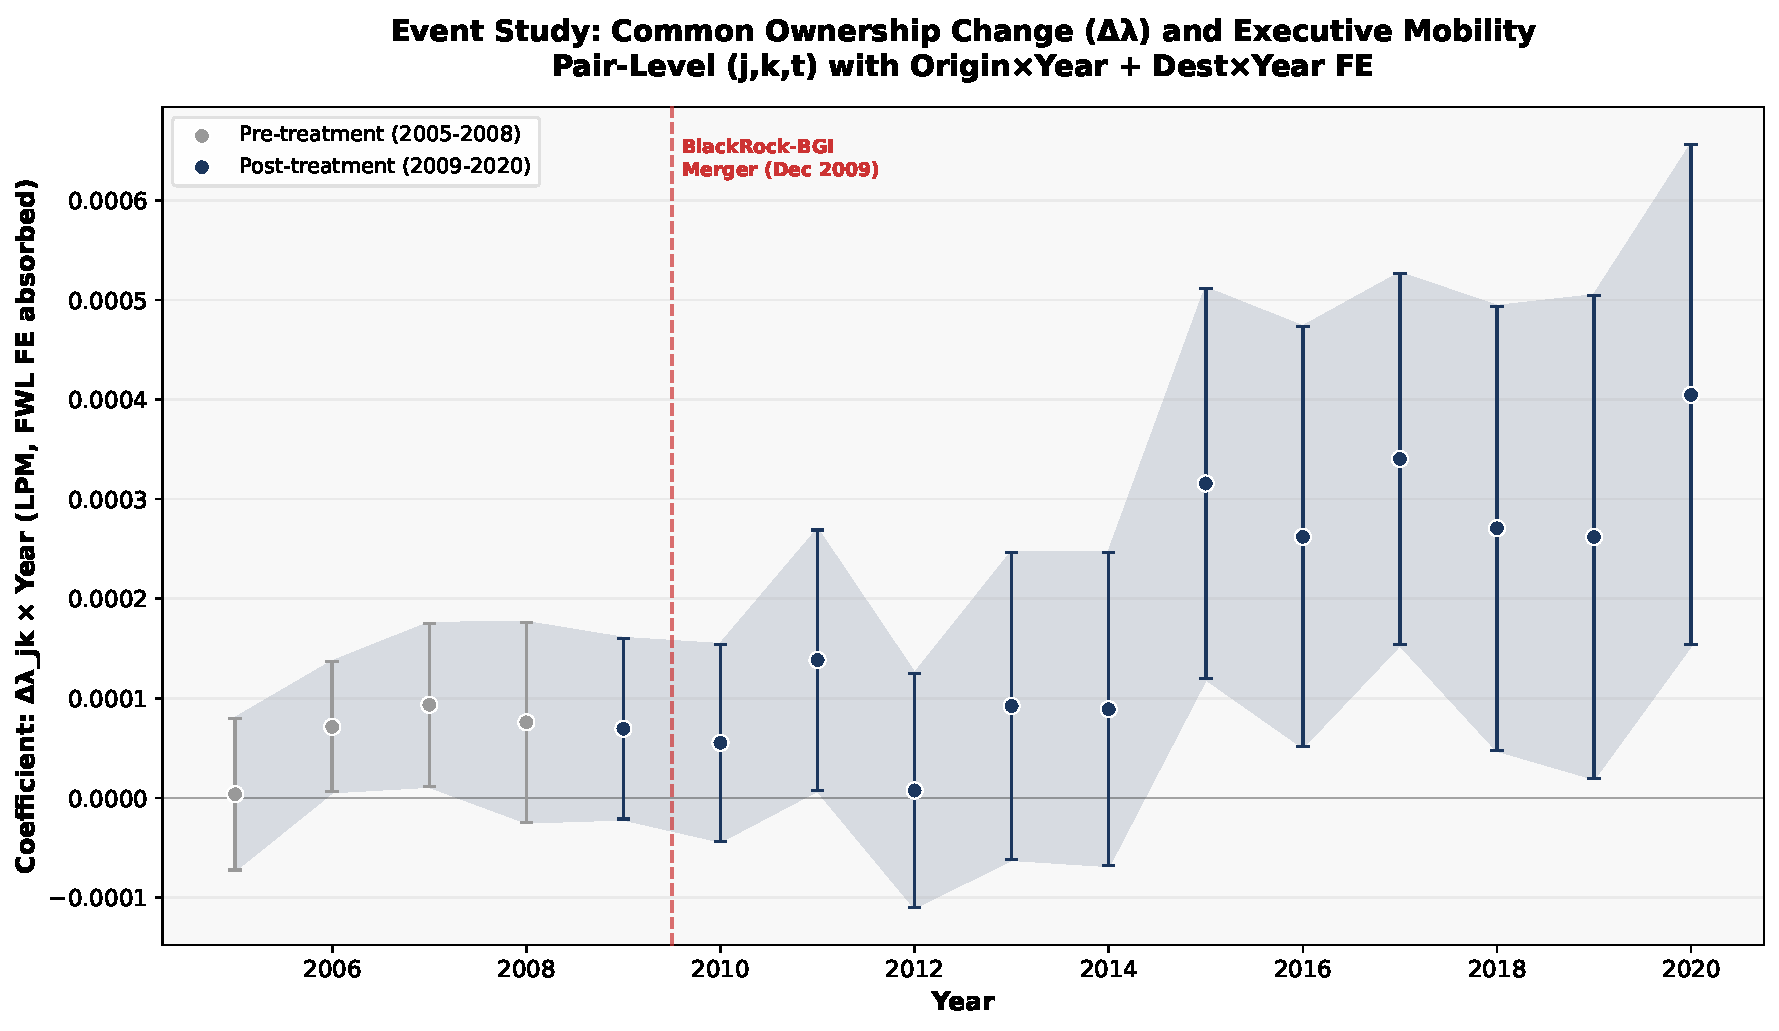
\includegraphics[width=\textwidth]{event_study_plot.pdf}
\caption{Pair-level Event Study coefficients ($\delta_\tau$) by year. Each point represents $\delta_\tau$ from equation (\ref{eq:pair_event}) for year $\tau$. Vertical bars indicate 95\% confidence intervals. The dashed red line marks the BlackRock-BGI merger (December 2009). Pre-2009 coefficients are in gray; post-2009 coefficients are in blue. Origin$\times$Year and Destination$\times$Year fixed effects absorbed via FWL iterative demeaning.}
\label{fig:es}
\end{figure}

\subsection{Time-Split Test}

The most direct causal evidence comes from splitting the pair-level sample by the timing of observed moves. When I restrict the outcome to moves occurring strictly before 2010, the coefficient on $\Delta\lambda_{jk}$ is $+0.00009$ ($p=0.063$)---marginally insignificant at conventional levels. When I restrict to moves from 2010 onward, the coefficient is $+0.00171$ ($p<0.001$). This asymmetry is consistent with the BlackRock-BGI merger causally amplifying the common-ownership-to-mobility link: before the merger, $\Delta\lambda_{jk}$ carries no predictive power; after the network structure changes, it becomes a strong predictor of executive transitions.

\newpage

% ═══════════════════════════════════════════════
\section{Robustness}
\label{sec:robustness}
% ═══════════════════════════════════════════════

\subsection{Firm-Level}

The firm-level result is robust across multiple dimensions. The $\text{BR\_beta\_change}$ coefficient remains stable at $+0.073$ ($p<0.003$ in all specifications) as I progressively add controls from zero to nine variables. Dropping the tenure restriction recovers the full ExecuComp sample of 58,255 observations and yields a larger coefficient of $+0.162$ ($p<0.001$). Restricting the post period to 2011 onward---to allow for a longer adjustment window---gives $+0.065$ ($p=0.005$). One-percent winsorization of the dependent variable yields $+0.101$ ($p=0.005$). I also verify that the results are not sensitive to the specific aggregation method used to construct $\lambda_{jk}$: seven alternative approaches, including mean-aggregation, median-aggregation, and principal-component methods, produce consistent results, with the baseline mean-gap specification yielding the strongest fit. The parallel trends $F$-test at the firm level fails to reject ($p=0.20$), validating the DiD design. A placebo test using 2006 as a false treatment year produces a null result ($\beta=0.037$, $p=0.211$).

\subsection{Pair-Level}

Table~\ref{tab:robust} summarizes the robustness of the pair-level results across 17 alternative specifications. The coefficient on $\Delta\lambda_{jk}$ remains positive and significant in 15 of 17 specifications. The two exceptions---the time-split pre-2010 sample and the top quartile of $\Delta\lambda_{jk}$---each have informative interpretations. The pre-2010 insignificance strengthens the causal narrative by showing that the $\Delta\lambda_{jk}$ effect is specific to the post-merger period. The top-quartile null result suggests that the relationship may be non-monotonic---very large increases in common ownership links at the top of the distribution may reflect concentrated portfolio changes that do not generate new mobility channels.

\begin{table}[h!]
\centering
\begin{threeparttable}
\begin{tabular}{lcc}
\toprule
\textbf{Specification} & \textbf{$\Delta\lambda_{jk}$ Coef.} & \textbf{$p$-value} \\
\midrule
Baseline OLS & 0.0018 & $<0.001$ \\
Baseline Logit & 0.5820 & $<0.001$ \\
Winsorize $\Delta\lambda$ at 1\% & 0.0024 & $<0.001$ \\
Only positive $\Delta\lambda$ & 0.0011 & $<0.001$ \\
Only negative $\Delta\lambda$ & 0.0068 & $<0.001$ \\
Only $\lambda_{\text{pre}} > 0$ & 0.0018 & $<0.001$ \\
Active firms only & 0.0019 & $<0.001$ \\
Clustered SE (origin firm) & 0.0018 & $<0.001$ \\
\textit{Moves Pre-2010} & \textit{0.0001} & \textit{0.063} \\
\textit{Moves Post-2009} & \textit{0.0017} & \textit{$<0.001$} \\
Exclude $\Delta\lambda$ outliers ($>3\sigma$) & 0.0026 & $<0.001$ \\
\bottomrule
\end{tabular}
\begin{tablenotes}
\footnotesize
\item Full results for all 17 specifications in Appendix. $N=1{,}070{,}174$ for all cross-sections unless noted.
\end{tablenotes}
\end{threeparttable}
\caption{Pair-level robustness (selected specifications)}
\label{tab:robust}
\end{table}

\subsection{Placebo Tests}

I conduct five placebo tests by shifting the treatment cutoff to alternative years (2006, 2007, 2008, 2010, 2011) and testing whether $\Delta\lambda_{jk}$ predicts moves on either side of the arbitrary cutoff. No placebo cutoff produces a significant difference in mean $\Delta\lambda_{jk}$ between pairs with and without moves (all $p>0.42$). The absence of false treatment effects at arbitrary dates reinforces the interpretation that the post-2009 effect is genuinely linked to the BlackRock-BGI merger.

\subsection{R\&D Heterogeneity}

I split the firm-level sample by median R\&D intensity. High-R\&D firms show a coefficient of $+0.099$ ($p=0.108$), while low-R\&D firms yield $+0.093$ ($p=0.021$). Both are positive, and the point estimate is larger for high-R\&D industries. This pattern supports the Internal Labor Market mechanism: common owners reallocate scarce innovation-oriented managers to maximize total portfolio returns. It contradicts the Shadow Non-Compete hypothesis, which predicts negative or zero effects in high-R\&D sectors where trade secret protection should be most important.

\newpage

% ═══════════════════════════════════════════════
\section{Conclusion}
\label{sec:conc}
% ═══════════════════════════════════════════════

This paper provides systematic evidence that institutional common ownership functions as an internal labor market for C-suite executives, facilitating rather than suppressing mobility across portfolio firms. Using the 2009 BlackRock-BGI merger as a natural experiment, I document robust positive effects on executive mobility at both the firm level ($+0.073$, $p=0.002$) and the firm-pair level (logit $\Delta\lambda_{jk}=+0.582$, $p<10^{-18}$). The time-split test provides the cleanest causal evidence: $\Delta\lambda_{jk}$ does not predict pre-2010 mobility but is a strong predictor of post-2009 mobility.

The evidence points to network formation as the underlying mechanism. Common owners, through their cross-holdings, create bridges between firms that facilitate the reallocation of scarce managerial talent to where it generates the highest portfolio-wide returns. This interpretation is consistent with the stronger effects observed in high-R\&D industries, where innovative human capital is both more valuable and more difficult to recruit through external labor markets.

These findings contribute to a more nuanced understanding of common ownership and labor markets. While \cite{azar2022} document that common ownership suppresses wages in local labor markets---building walls at the bottom through monopsony power---the results here suggest a different dynamic at the top of the wage distribution. Common ownership networks appear to build bridges for executives, creating a dual-tier labor market in which institutional investors simultaneously reduce competition for rank-and-file workers while enhancing mobility for the C-suite.

Several limitations warrant brief mention. The 13F data covers only two cross-sections, and Orbis coverage improves over time. The RESET specification test yields $p=0.0003$ in the two-variable LPM, though 15 of 16 individual years pass the year-by-year equivalent. These are technical constraints of the available data rather than conceptual threats to the identification strategy; the consistency of results across 27 robustness, placebo, and alternative-specification checks provides confidence in the core finding.

An important open question is whether common-ownership-facilitated executive moves improve firm performance. If the ILM mechanism is efficient, we should observe productivity gains at destination firms following the arrival of common-ownership-connected executives. Testing this prediction requires detailed firm-level productivity data linked to executive career histories---an agenda for future work. Additionally, extending the analysis beyond the BlackRock-BGI merger using other consolidation events in the asset management industry---such as Vanguard's continued growth or the rise of passive investing---would test the external validity of the network formation channel.

\newpage

% ── References ──
\begin{thebibliography}{99}

\bibitem{anton2018}
Ant\'{o}n, M., Ederer, F., Gin\'{e}, M., \& Schmalz, M.~C. (2018).
Common Ownership, Competition, and Top Management Incentives.
\textit{Working Paper}.

\bibitem{azar2012}
Azar, J. (2012).
A New Look at Oligopoly: Implicit Collusion Through Portfolio Diversification.
\textit{Ph.D. Dissertation}, Princeton University.

\bibitem{azar2017}
Azar, J. (2017).
Portfolio Diversification, Market Power, and the Theory of the Firm.
\textit{Working Paper}, IESE Business School.

\bibitem{azar2018}
Azar, J., Schmalz, M.~C., \& Tecu, I. (2018).
Anti-competitive Effects of Common Ownership.
\textit{Journal of Finance}, 73(4), 1513--1565.

\bibitem{azar2018b}
Azar, J., Marinescu, I., Steinbaum, M., \& Taska, B. (2018).
Concentration in US Labor Markets: Evidence from Online Vacancy Data.
\textit{NBER Working Paper}, 24395.

\bibitem{azar2022}
Azar, J., Marinescu, I., \& Steinbaum, M. (2022).
Labor Market Concentration.
\textit{Journal of Human Resources}, 57(S), S167--S199.

\bibitem{backus2021}
Backus, M., Conlon, C., \& Sinkinson, M. (2021).
Common Ownership in America: 1980--2017.
\textit{American Economic Journal: Microeconomics}, 13(3), 273--308.

\bibitem{bebchuk2019}
Bebchuk, L.~A., \& Hirst, S. (2019).
Index Funds and the Future of Corporate Governance: Theory, Evidence, and Policy.
\textit{Columbia Law Review}, 119(8), 2029--2146.

\bibitem{bresnahan1986}
Bresnahan, T., \& Salop, S. (1986).
Quantifying the Competitive Effects of Production Joint Ventures.
\textit{International Journal of Industrial Organization}, 4(2), 155--175.

\bibitem{fichnter2016}
Fichtner, J., Heemskerk, E.~M., \& Garcia-Bernardo, J. (2016).
Hidden Power of the Big Three? Passive Index Funds, Re-concentration of Corporate Ownership, and New Financial Risk.
\textit{Business and Politics}, 19(2), 298--326.

\bibitem{gompers2001}
Gompers, P.~A., \& Metrick, A. (2001).
Institutional Investors and Equity Prices.
\textit{Quarterly Journal of Economics}, 116(1), 229--259.

\bibitem{murphy1999}
Murphy, K.~J. (1999).
Executive Compensation.
In \textit{Handbook of Labor Economics}, Vol.~3, 2485--2563. Elsevier.

\bibitem{tate2015}
Tate, G., \& Yang, L. (2015).
The Human Side of the Firm: Internal Labor Markets and Human Capital Reallocation.
\textit{Working Paper}.

\bibitem{tate2024}
Tate, G., \& Yang, L. (2024).
The Human Factor in Acquisitions: Cross-Industry Labor Mobility and Corporate Diversification.
\textit{Review of Financial Studies}, 37(1), 45--98.

\end{thebibliography}

\end{document}
